\documentclass[conference]{IEEEtran}
\usepackage[utf8]{inputenc}
\usepackage[T1]{fontenc}
\usepackage{graphicx}
\usepackage{booktabs}
\usepackage{amsmath}
\usepackage{siunitx}
\usepackage{url}
\usepackage{tabularx}
\graphicspath{{figs/}}

\begin{document}

\title{SudokuScan: From a Photograph of a Printed Puzzle\\to a Digital $9\times9$ Grid}

\author{\IEEEauthorblockN{Efe G\"unay}
\IEEEauthorblockA{Student no.\ 042101085\\
COMP 482 Computer Vision, MEF University, Fall 2026}}

\maketitle

\begin{abstract}
SudokuScan reads a phone photograph of a printed sudoku and returns the puzzle as a $9\times9$
grid. The four outer corners are selected automatically from Harris corner candidates, the
grid is rectified with an affine and a projective model, the 81 cells are split, classified as
empty or filled, and read with Tesseract, and the result is checked against the sudoku rules.
On 12 personal phone photos the system reaches a mean corner error of 0.35\,\% of the puzzle
side, 98.9\,\% cell accuracy and 100\,\% robustness; on the 20-image development set 0.50\,\%
and 99.8\,\%. Measured on the same photos, an affine rectification reads every cell only while
the relative depth spread of the puzzle stays below about 0.1, which is the weak-perspective
limit; beyond it a homography is required.
\end{abstract}

\section{Introduction}
A printed puzzle photographed with a phone is a plane seen through a perspective camera. The
photo may be oblique, rotated in-plane by up to $\pm30^\circ$, unevenly lit and surrounded by
other text, tables or a second rectangle. The task is to find the puzzle without any manual
input, undo the projection, and read the printed givens.

The pipeline (Fig.~\ref{fig:pipeline}) has six stages, each a separate function in
\texttt{sudoku\_scan.py}: (1) illumination-normalised preprocessing, (2) Harris corner
detection and automatic selection of the four outer corners, (3) rectification with three
models (A3, A4, H4), (4) a comparison of those models, (5) cell extraction, empty-cell detection
and OCR, and (6) a validity check. The program never crashes on an input: any failure produces
a result file with \texttt{"verdict": "not\_found"}. The slowest image takes 3.4\,s on a laptop
CPU (limit 20\,s).

\begin{figure*}[t]
\centering
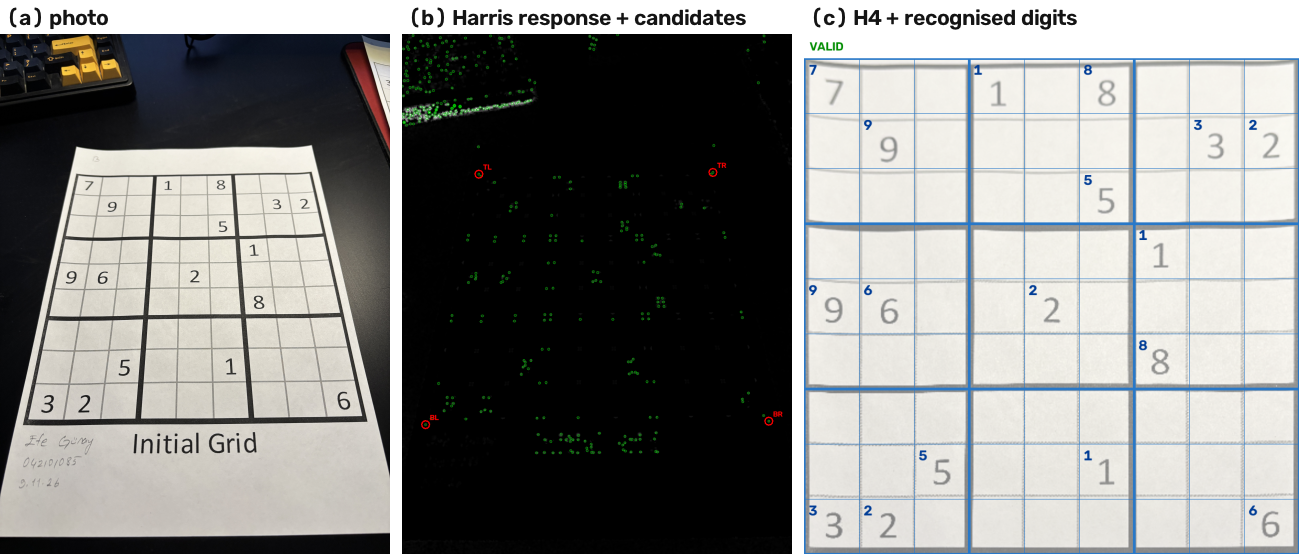
\includegraphics[width=\textwidth]{fig_pipeline.png}
\caption{Pipeline on IMG\_8797 (moderately oblique, keyboard and a second sheet in the frame).
(b) Harris response with all candidates (green) and the four selected corners (red). (c) The H4
rectification with cell boundaries and the recognised digits (blue).}
\label{fig:pipeline}
\end{figure*}

\section{Corner detection}
\subsection{Preprocessing}
Images are downscaled so that the long side is 1200\,px (the corners are later mapped back with
$x_{\mathrm{orig}} = (x+0.5)/s - 0.5$), converted to grey and smoothed with a Gaussian whose
size is 0.3\,\% of the width. Uneven light is removed by dividing the image by a background
estimate: a morphological closing with a kernel of 2\,\% of the width (wider than any ink
stroke) erases the ink and keeps the paper brightness, shadows included. After division the
paper is close to 1 everywhere and ink keeps the same relative darkness inside and outside a
shadow. All sizes are fractions of the image width, so the same code serves a 1600\,px and a
5712\,px input.

\subsection{Harris candidates}
\texttt{cv2.cornerHarris} is applied to the normalised image ($\mathrm{blockSize}=5$,
$\mathrm{ksize}=3$, $k=0.04$). Pixels with $R > 0.01\,R_{\max}$ are kept and non-maximum
suppression keeps a pixel only if it equals the maximum of its $9\times9$ neighbourhood
(implemented as a comparison with the dilated response). A photo yields about 600 candidates:
grid intersections, digit strokes, background text and objects (Fig.~\ref{fig:pipeline}b).

\subsection{Selecting the four corners}
Contours are used only to find the puzzle \emph{region}; the coordinates come from Harris.
\begin{enumerate}
\item The normalised image is thresholded (ink $<220$) and every external or internal contour
covering at least 2\,\% of the frame is approximated by its convex hull and a 4-vertex polygon.
\item Each quadrilateral is tested by warping it to $450\times450$\,px and measuring the ink
profile of the 10 horizontal and 10 vertical lines that a sudoku must have every 50\,px. The
profile is measured separately in each of the 9 cell-wide strips with a $\pm6$\,px window, so
a slightly curved line still counts. The \emph{box score} is the weakest of the four box lines
(positions 0, 3, 6, 9); a candidate needs a box score $\geq 0.6$ and the strongest one wins.
A single $3\times3$ box fails because its inner lines are thin cell lines; the paper sheet or
another rectangle fails because its inner lines do not fall at the thirds.
\item For each corner of the winning region the nearest Harris candidate within a quarter
cell is taken; if any corner has none, the image is \texttt{not\_found}.
\item The corners are ordered TL, TR, BR, BL by their angle around the centroid (TL is the one
closest to $-135^\circ$; valid for in-plane rotation below $45^\circ$) and refined with
\texttt{cv2.cornerSubPix} on the full-resolution image.
\end{enumerate}
The box-line rule replaced a first version that scored all 20 lines. That version failed on
real photos (Section~\ref{sec:failures}): at a 0.21 downscale the thin lines almost vanish, so
the true grid scored zero and a single box or the paper sheet won.

\subsection{Parameter study}
Fig.~\ref{fig:params} varies one parameter at a time on the 12 annotated photos. The number of
candidates falls with every parameter, but only $\mathrm{blockSize}$ moves the corner error
substantially: a larger window shifts the response peak inwards from the outer corner, from
0.16\,\% at $\mathrm{blockSize}=3$ to 1.29\,\% at 13. Small windows are more accurate but too
noisy to find the corners in every image (6/12 at 2, 8/12 at 3). $\mathrm{ksize}$ and $k$ change
the error by less than 0.1\,\% and mainly affect reliability ($k\geq0.06$ loses two images).
The threshold sets the number of candidates (1287 at 0.001, 82 at 0.3) and starts losing
corners above 0.01. The chosen values are the most selective ones that still find the corners
in all 12 images.

\begin{figure*}[t]
\centering
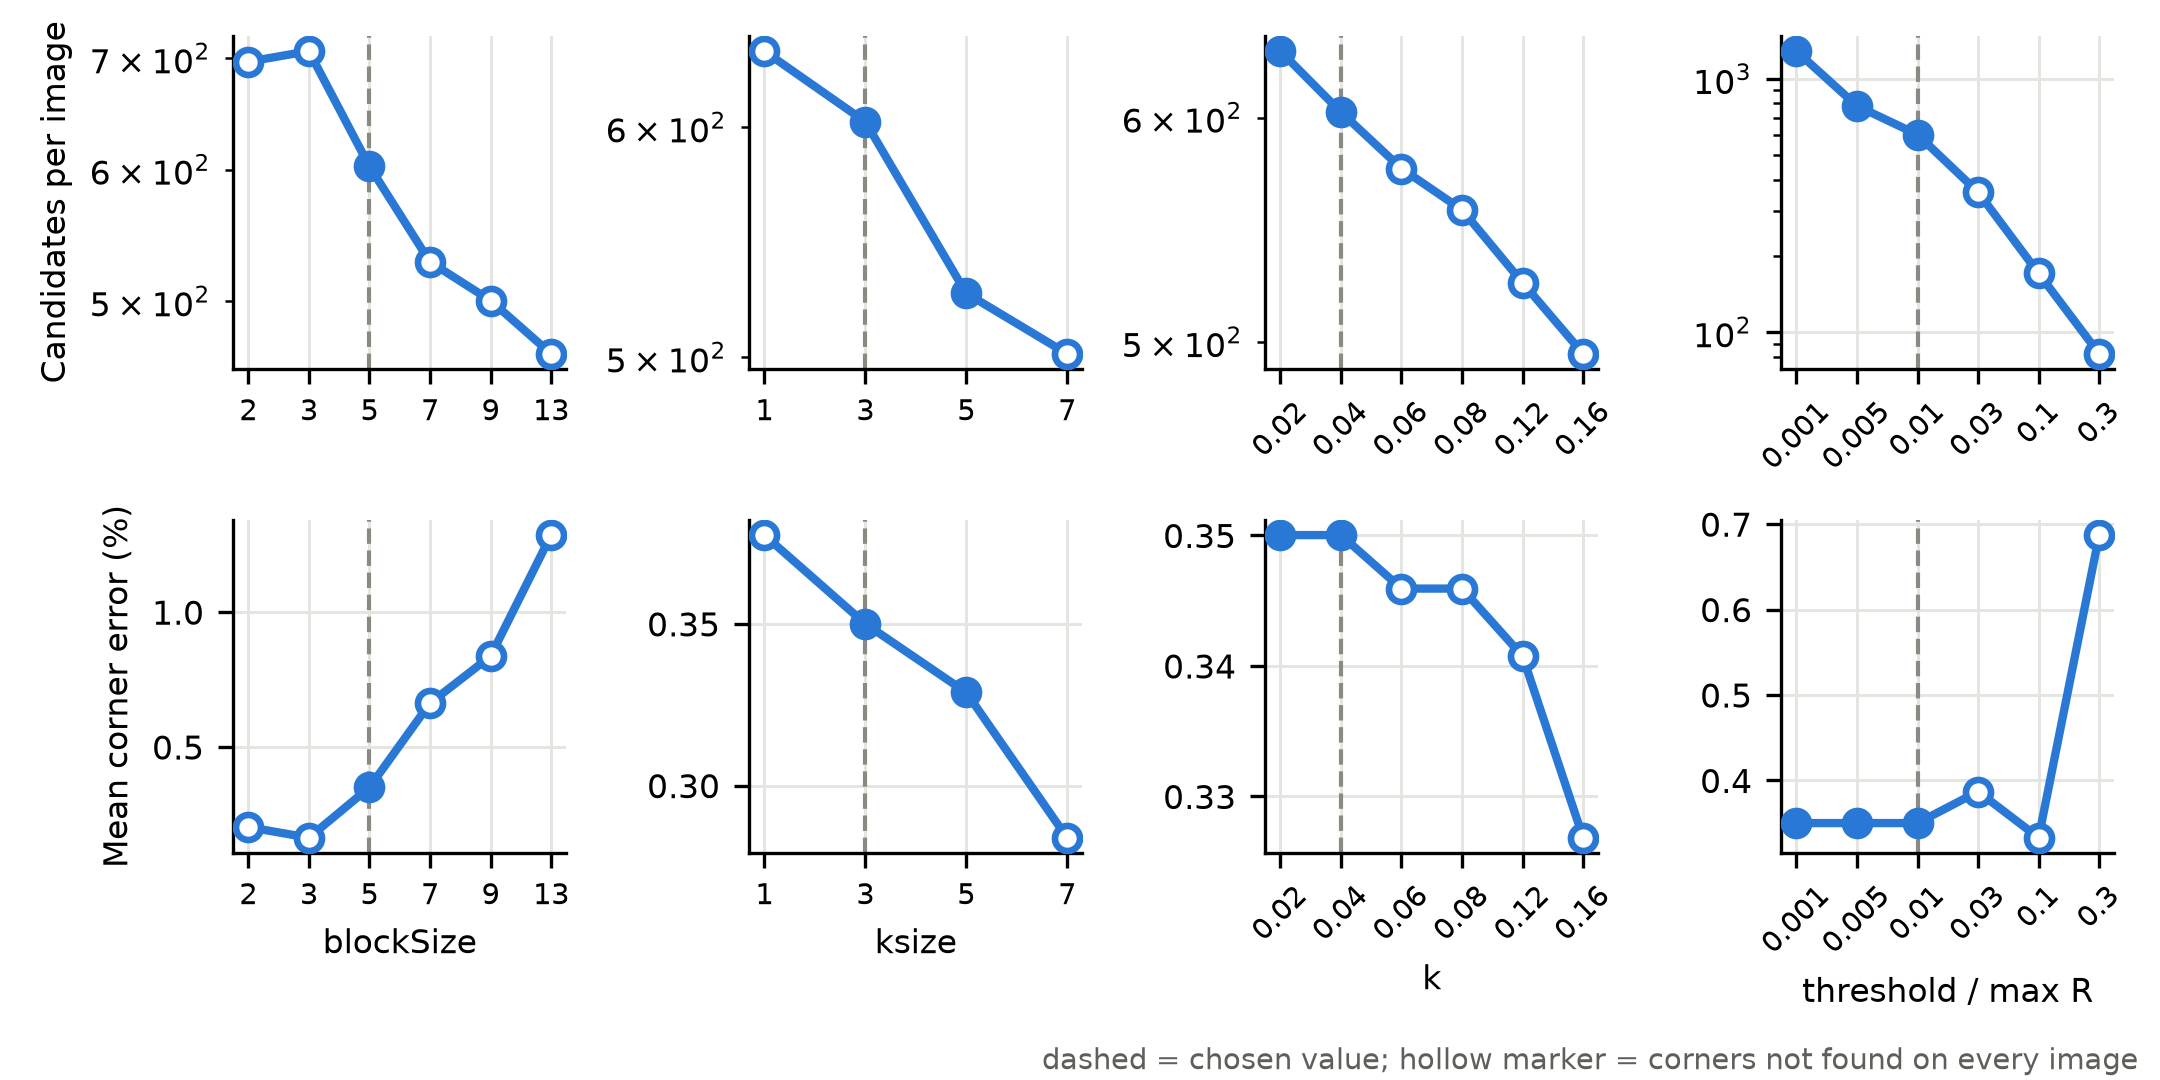
\includegraphics[width=0.92\textwidth]{fig_param_study.png}
\caption{Harris parameter study on the 12 personal photos (one parameter varied, the others at
the chosen value, dashed). Top: candidates per image (log scale). Bottom: mean corner error.
Hollow markers: the corners were not found in every image.}
\label{fig:params}
\end{figure*}

\section{Rectification}
The corners are mapped to $(-0.5,-0.5)$, $(449.5,-0.5)$, $(449.5,449.5)$, $(-0.5,449.5)$:
pixel centres are integers in OpenCV, so these are the outer edges of a $450\times450$ image
and every cell is exactly $50\times50$\,px.

\textbf{A3} (\texttt{getAffineTransform} from TL, TR, BL). An affine map
$\mathbf{x}' = A\mathbf{x} + \mathbf{t}$ has 6 degrees of freedom; each point pair gives two
equations, so three pairs determine it exactly. BR is not used and lands where the model sends
it; its distance from $(449.5,449.5)$ is the \emph{A3 fourth-corner error}.

\textbf{A4} (\texttt{estimateAffine2D} on all four corners). Eight equations for six unknowns
are solved in the least-squares sense. \texttt{estimateAffine2D} is a RANSAC estimator; with a
reprojection threshold of $10^6$ every corner is an inlier and the final Levenberg--Marquardt
step is the plain least-squares fit (it matches \texttt{numpy.linalg.lstsq} to 0.007\,px). The
RMS distance of the four mapped corners from the target is the \emph{A4 residual}.

\textbf{H4} (\texttt{getPerspectiveTransform}). A homography is a $3\times3$ matrix defined up
to scale: 8 degrees of freedom, so four point pairs (no three collinear) determine it exactly.
On every image the four corners map onto the target within $4\times10^{-3}$\,px.

An affine map keeps parallel lines parallel and preserves ratios along a line, so it cannot
represent the converging grid lines of an oblique view. A homography maps the line at infinity
to a finite line: the two vanishing points of the grid become points at infinity again, and the
grid becomes square. On the personal photos the A3 fourth-corner error ranges from 21 to
297\,px and the A4 residual from 5 to 54\,px (Table~\ref{tab:stage4}).

\section{Affine versus homography}
\textbf{Obliqueness.} Two measures are used: the largest ratio between opposite sides of the
detected quadrilateral, and the relative depth spread $\Delta z/\bar z$ of the four corners. For
a plane, the third row of $H_4^{-1}$ gives each point's projective depth $w = h_{31}x + h_{32}y +
h_{33}$, which is proportional to its camera depth; $\Delta z/\bar z = (w_{\max}-w_{\min})/\bar
w$. The two agree ($r=0.90$), but $\Delta z/\bar z$ is better when tilt and rotation combine
(IMG\_8801: side ratio 1.38, $\Delta z/\bar z = 0.58$).

\textbf{Measures.} (i) The A3 fourth-corner error and A4 residual. (ii) Grid straightness: each
of the 10+10 grid lines is located in each of the 9 cell-wide strips of the rectified image
(180 segments) from an ink-profile peak, and its distance to the ideal 50\,px position is
averaged. (iii) The same OCR stage run on A3, A4 and H4.

\begin{table}[t]
\centering
\caption{Affine versus homography on the 12 personal photos, sorted by obliqueness.}
\label{tab:stage4}
\setlength{\tabcolsep}{3pt}
\footnotesize
\begin{tabular}{@{}lcccccc@{}}
\toprule
 & side & & A3 err & A4 RMS & line dev.\,(px) & cell acc.\,(\%)\\
Image & ratio & $\frac{\Delta z}{\bar z}$ & (px) & (px) & A3/A4/H4 & A3/A4/H4\\
\midrule
8802 & 1.05 & .05 & 21 & 5 & 5.1/3.9/0.7 & 95/100/96\\
8795 & 1.06 & .06 & 28 & 7 & 6.2/4.0/1.3 & 93/100/100\\
8800 & 1.07 & .09 & 33 & 8 & 9.0/4.8/1.7 & 78/100/100\\
8794 & 1.09 & .09 & 39 & 9 & 8.1/6.0/2.2 & 81/100/99\\
8805 & 1.10 & .11 & 45 & 11 & 8.3/6.7/1.2 & 84/95/100\\
8803 & 1.12 & .11 & 52 & 12 & 8.6/5.8/1.1 & 72/91/100\\
8804 & 1.18 & .17 & 79 & 18 & 12.1/8.4/1.2 & 65/86/100\\
8796 & 1.28 & .25 & 125 & 27 & 14.5/11.6/2.1 & 53/63/99\\
8798 & 1.33 & .29 & 148 & 32 & 14.6/12.6/0.6 & 64/58/99\\
8801 & 1.38 & .58 & 206 & 47 & 13.8/14.6/1.6 & 73/67/100\\
8797 & 1.46 & .38 & 208 & 42 & 14.1/10.7/1.6 & 68/70/100\\
8799 & 1.66 & .50 & 297 & 54 & 15.3/13.9/7.0 & 49/47/94\\
\midrule
mean & & & & & & 73/82/99\\
\bottomrule
\end{tabular}
\end{table}

\begin{figure}[t]
\centering
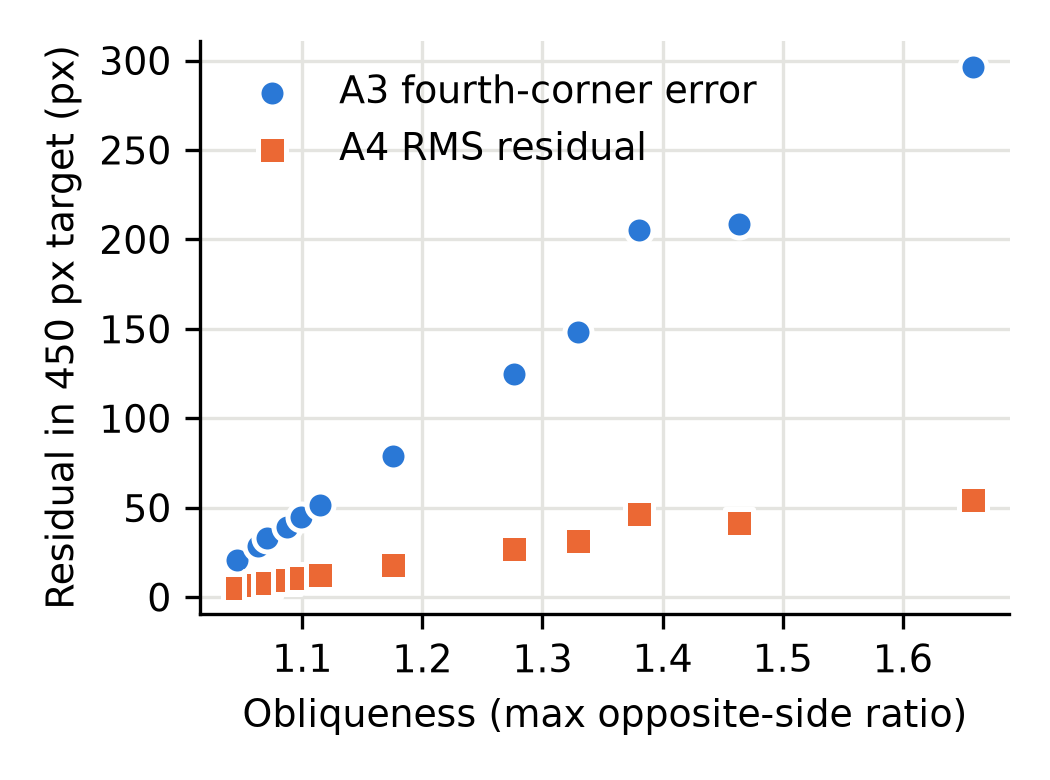
\includegraphics[width=\columnwidth]{fig_residuals.png}\\[2pt]
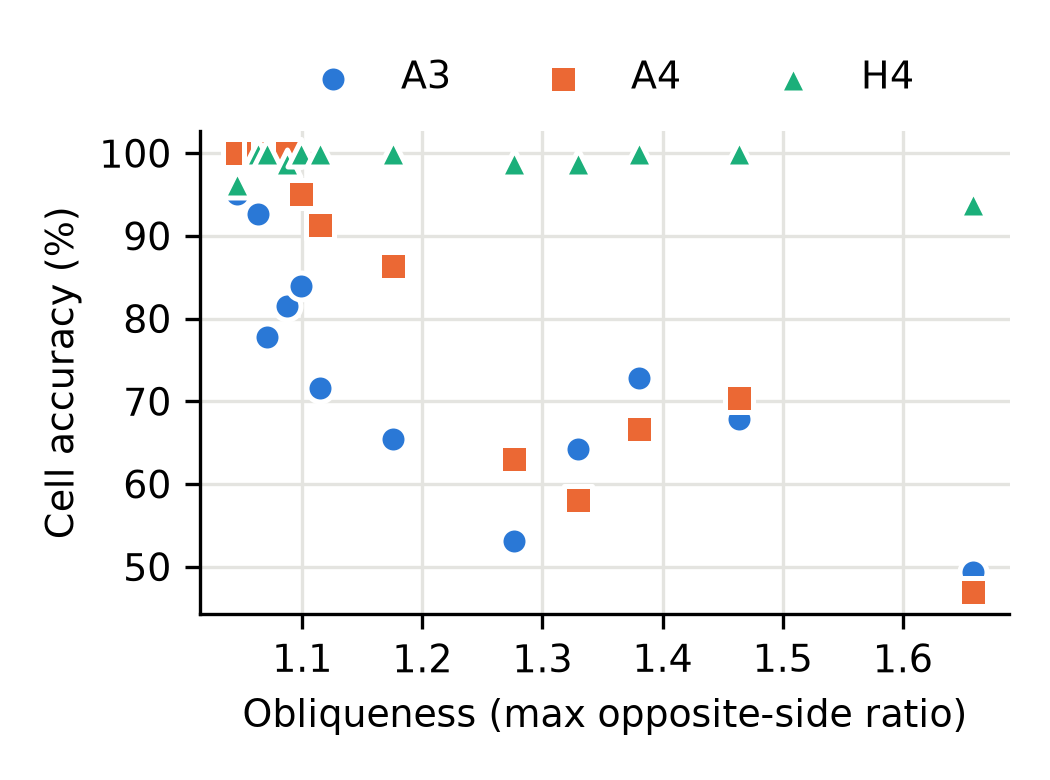
\includegraphics[width=\columnwidth]{fig_cell_accuracy.png}
\caption{Top: A3 fourth-corner error and A4 residual against obliqueness. Bottom: OCR cell
accuracy of the same recognition stage on A3, A4 and H4.}
\label{fig:stage4}
\end{figure}

\begin{figure*}[t]
\centering
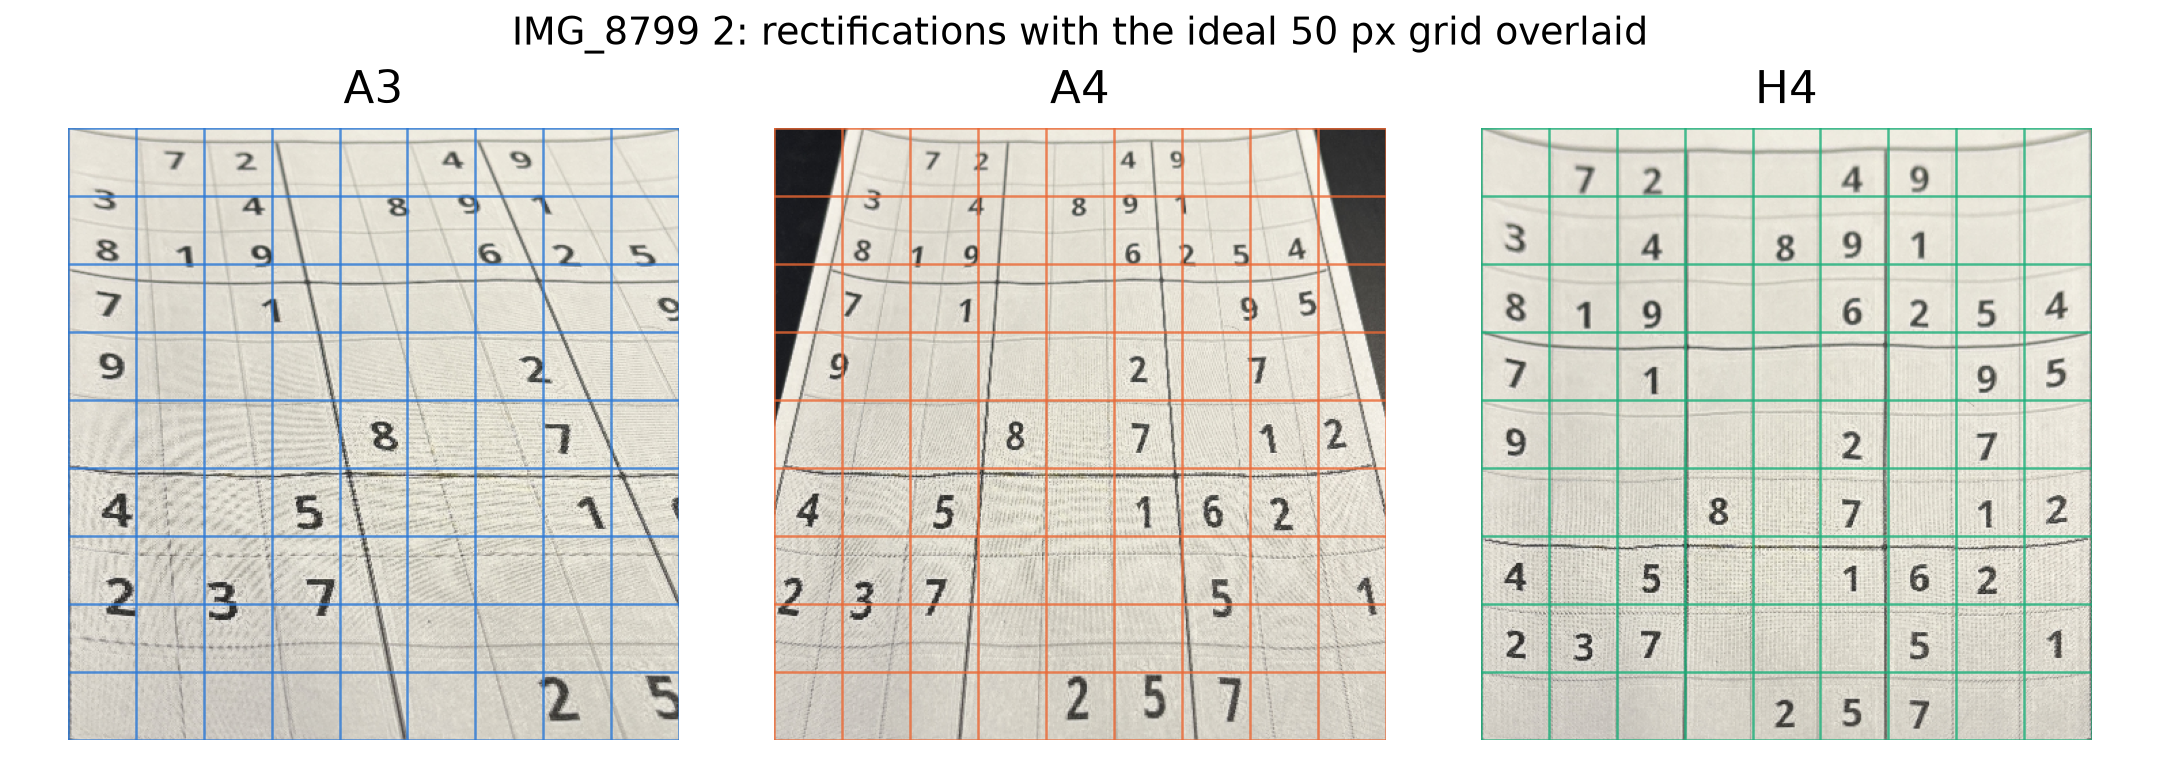
\includegraphics[width=0.85\textwidth]{fig_side_by_side.png}
\caption{The most oblique photo (IMG\_8799, side ratio 1.66) rectified with A3, A4 and H4; the
ideal 50\,px grid is overlaid. Only H4 brings the grid lines onto the ideal positions; the top
lines stay curved because the page is curled.}
\label{fig:sidebyside}
\end{figure*}

\textbf{Results.} (1) The residuals grow linearly with depth spread: A4 RMS $\approx
93\,\mathrm{px}\times\Delta z/\bar z + 1.9$\,px ($r=0.97$) on the photos and $98\,\mathrm{px}
\times\Delta z/\bar z$ ($r=0.99$) on the synthetic set, so the residual is a property of the
geometry, not of the images. The A3 error is a median $4.3\times$ the A4 residual: A3 fits
three corners exactly and extrapolates to BR with no constraint there (Fig.~\ref{fig:stage4}).
(2) H4 grid lines stay within 0.6--2.2\,px of the ideal at every angle (7.0\,px on the curled
IMG\_8799). Using the annotated corners gives the same values, so this is the limit of the
planar model on real paper (curl, lens distortion), not corner error; on the perfectly planar
synthetic images it is 0.05\,px. (3) With A4 the OCR is 100\,\% correct up to $\Delta z/\bar z
\approx 0.09$, drops to 91--95\,\% at 0.11, to 86\,\% at 0.17 and to 47--70\,\% beyond 0.24, in
step with A4 grid lines exceeding the 7\,px cell margin. A3 never reaches 100\,\%. Even the most
frontal hand-held photo has $\Delta z/\bar z = 0.05$.

\textbf{Conclusion.} An affine model is acceptable only while the depth variation across the
puzzle is small compared with its distance: in our data A4 reads every cell up to $\Delta
z/\bar z \approx 0.09$ (side ratio $\approx1.09$, a camera tilt of roughly $10^\circ$) and fails
quickly beyond 0.1. This is the weak-perspective condition: perspective divides each point by
its own depth $z$; weak perspective divides all points by one average depth $\bar z$, which is
valid when $\Delta z \ll \bar z$ (rule of thumb $\Delta z<\bar z/10$). Under it the image of a
plane is an affine map, parallel lines stay parallel and the projective row $(h_{31},h_{32})$
of the homography vanishes. Tilting the camera increases $\Delta z/\bar z$, moves the vanishing
points in from infinity and increases the affine error proportionally. The measured
break-even, $\Delta z/\bar z\approx0.1$, is that rule-of-thumb limit.

\section{Recognition}
\textbf{Cells and margin.} The H4 image is split into 81 cells of $50\times50$\,px and a margin
is cut from every side. A sweep of the margin (Table~\ref{tab:margin}) shows grid-line remnants
reaching the crop below 6\,px; between 7 and 10\,px the empty-cell decision is best on both
sets, and above 12\,px large digits start to be cut. We use 7\,px: the smallest value at the
optimum, which leaves the most digit area.

\begin{table}[t]
\centering
\caption{Empty-cell F1 of the filled/empty criterion against the cell margin (detected corners).}
\label{tab:margin}
\footnotesize
\begin{tabular}{@{}lccccccc@{}}
\toprule
margin (px) & 2 & 4 & 5 & 6 & 7 & 10 & 14\\
\midrule
devset & .939 & .993 & .999 & 1.00 & 1.00 & 1.00 & 1.00\\
personal & .845 & .970 & .990 & .993 & .994 & .994 & .988\\
\bottomrule
\end{tabular}
\end{table}

\textbf{Empty or filled.} The H4 image is flattened like Stage~1 (closing kernel 15\,px) and
thresholded at 0.75 of the local paper brightness. In each cell crop the connected components
that touch the crop border and are thinner than 15\,\% of it are discarded as line remnants. The
cell is filled only if the largest remaining component covers at least 3\,\% of the crop and is
at least 35\,\% of its height. This decision is made before OCR is called.

\textbf{Cell preparation.} For a filled cell, the digit's components are kept, everything else
is painted white, the digit is cropped, scaled to 48\,px height with cubic interpolation,
contrast-stretched and padded with 20\,px of white. Keeping the grey, anti-aliased digit
matters: a first version that binarised the digit had 11 errors on the 565 devset digits, the
grey version 4. Tesseract's LSTM model was trained on smooth scanned text and stumbles on
staircase edges.

\textbf{OCR configuration.} Table~\ref{tab:ocr} reports digit accuracy on the 356 filled cells
of the personal set (annotated corners). Preparation is the largest factor (best raw
configuration 80.1\,\%, prepared 97.8--98.0\,\%). Single-character mode (\texttt{--psm 10}) and
the line modes (6, 7) are close; word and raw-line modes (8, 13) fall to 91\,\% because they
read thin 1s as 4s. We use \texttt{--oem 1 --psm 10} with the whitelist \texttt{123456789} and a
second attempt with \texttt{--psm 13} when nothing is returned (98.0\,\%).

\begin{table}[t]
\centering
\caption{Digit accuracy (\%) on 356 filled cells for page-segmentation modes, with and without
the digit whitelist and the cell preparation.}
\label{tab:ocr}
\footnotesize
\begin{tabular}{@{}lccccc@{}}
\toprule
psm & 6 & 7 & 8 & 10 & 13\\
\midrule
prepared, whitelist & 97.8 & 94.7 & 91.3 & 94.9 & 91.3\\
prepared, no whitelist & 96.9 & 96.4 & 90.5 & 96.6 & 90.5\\
raw cell, whitelist & 80.1 & 76.7 & 48.0 & 77.0 & 48.0\\
\midrule
used: psm 10 $\rightarrow$ 13 & \multicolumn{5}{c}{98.0}\\
\bottomrule
\end{tabular}
\end{table}

\textbf{Confusions.} With detected corners, 8 of the 11 cell errors on the personal set are
digits that Tesseract does not read at all (8, 4, 9, 1, 7 returned as empty); the other three
are 5$\to$3, 2$\to$5 and 3$\to$2. Fig.~\ref{fig:ocrfail} shows the crops that still fail with
the annotated corners: five come from the curled IMG\_8799, where a bent grid line enters the
cell; two from IMG\_8802, the puzzle printed on a grey halftone, whose dots survive the
preparation.

\begin{figure}[t]
\centering
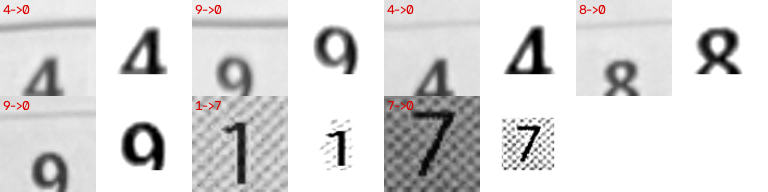
\includegraphics[width=\columnwidth]{fig_ocr_failures.png}
\caption{Remaining OCR failures (personal set, annotated corners): raw crop and prepared input,
true $\rightarrow$ predicted digit (0 = nothing read).}
\label{fig:ocrfail}
\end{figure}

\textbf{Validity.} Every row, column and $3\times3$ box is checked for repeated digits; repeated
cells are listed and drawn in red in the debug image (Fig.~\ref{fig:failures}c).

\section{Results}
Table~\ref{tab:results} gives the Section~7 metrics. Corner error is the mean distance to the
annotated corners as a percentage of the puzzle side.

\begin{table}[t]
\centering
\caption{Evaluation metrics (detected corners, full pipeline).}
\label{tab:results}
\setlength{\tabcolsep}{3.5pt}
\footnotesize
\begin{tabular}{@{}llcccccc@{}}
\toprule
set & cond. & $n$ & corner & cell acc. & empty & exact & robust\\
 & & & err.\,\% & \% & F1 & \% & \%\\
\midrule
devset & all & 20 & 0.50 & 99.81 & .998 & 90 & 100\\
 & C1 & 5 & 0.55 & 99.75 & 1.00 & 80 & 100\\
 & C2 & 9 & 0.45 & 99.73 & .996 & 89 & 100\\
 & C3 & 4 & 0.52 & 100.0 & 1.00 & 100 & 100\\
 & C4 & 6 & 0.42 & 99.59 & .994 & 83 & 100\\
 & C5 & 6 & 0.61 & 100.0 & 1.00 & 100 & 100\\
\midrule
personal & all & 12 & 0.35 & 98.87 & .989 & 58 & 100\\
 & C1 & 3 & 0.26 & 99.59 & .993 & 67 & 100\\
 & C2 & 5 & 0.26 & 98.27 & .979 & 40 & 100\\
 & C3 & 2 & 0.49 & 100.0 & 1.00 & 100 & 100\\
 & C4 & 2 & 0.45 & 98.15 & .993 & 50 & 100\\
 & C5 & 6 & 0.34 & 98.77 & .980 & 67 & 100\\
\bottomrule
\end{tabular}
\end{table}

The corners are found in all 32 images and are more accurate on the real photos than on the
synthetic ones (0.35 vs.\ 0.50\,\%), possibly because the 12-megapixel photos give the
sub-pixel refinement more detail than the blurred, noisy synthetic images. The cell accuracy is lower on the photos because of the two
failure modes above; oblique photos (C2) are hardest. The empty-cell F1 here is computed on the
final grid, so an unread digit counts as a false ``empty''; the empty/filled criterion alone
scores 0.994 on the photos and 1.00 on the devset (Table~\ref{tab:margin}). The personal set
has 12 photos of 3 puzzles; the conditions are not balanced (C3 and C4 have two images each).

\section{Failure analysis}\label{sec:failures}
Fig.~\ref{fig:failures} shows four failures, two of which led to changes in the method.

\textbf{(a) Region: a single box chosen (IMG\_8799, first version).} The photo is 5712\,px wide
and strongly oblique; after downscaling to 1200\,px the thin cell lines are broken dots, and
the page curl bends the horizontal lines. The first region score needed all 20 lines, so the
true grid scored zero and a $3\times3$ box with its four strong lines won. \emph{Stage:} corner
selection. \emph{Fix:} per-strip line search with a $\pm6$\,px window and the box-line score.

\textbf{(b) Region: the paper sheet chosen (IMG\_8804, intermediate version).} Selecting the
\emph{largest} candidate with box structure picked the sheet, whose edges and the printed grid
happen to give lines near its thirds. \emph{Stage:} corner selection. \emph{Fix:} choose the
candidate with the \emph{strongest} box lines instead of the largest one.

\textbf{(c) OCR misread changes the verdict (IMG\_8796).} A clear 5 is read as 3, creating a
duplicate in its row; the validity check correctly reports \texttt{invalid} and marks both
cells. \emph{Stage:} recognition. The validity check catches such errors only when they create a
conflict; a missed digit (read as empty) never does.

\textbf{(d) Page curl (IMG\_8799, final version).} The corners and region are right, but the
curled top of the page cannot be flattened by any $3\times3$ map (H4 line deviation 7\,px).
Bent lines enter the cells and five digits are not read. \emph{Stage:} rectification model.
A many-point homography or a local (piecewise) warp would be needed.

\begin{figure}[t]
\centering
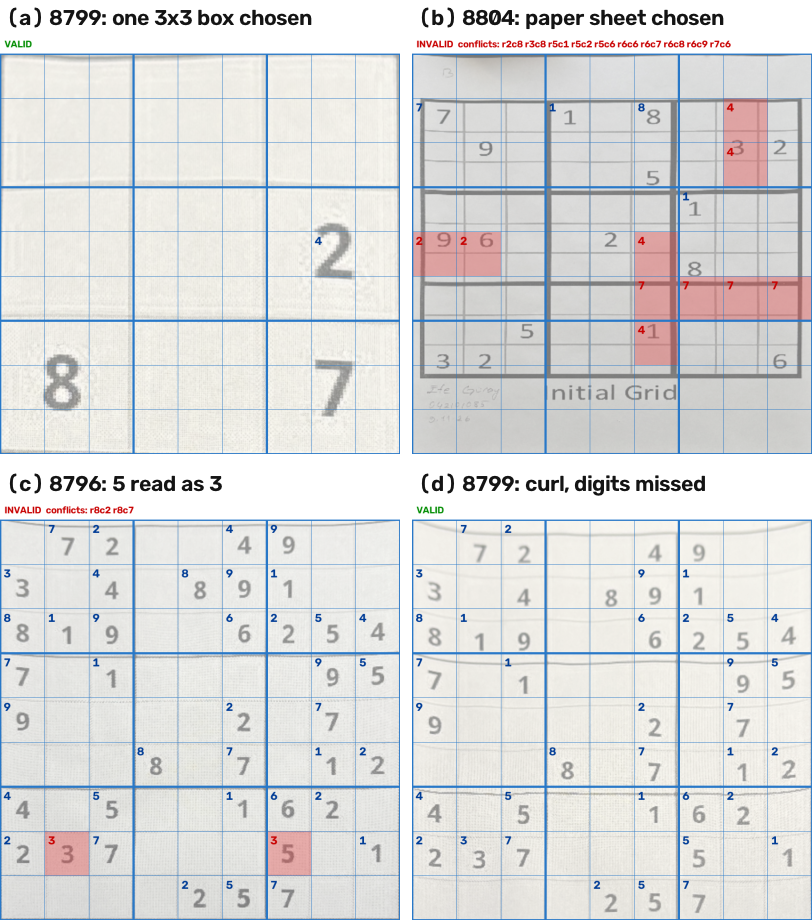
\includegraphics[width=\columnwidth]{fig_failures.png}
\caption{Failure cases (debug images: H4 rectification, recognised digits in blue, conflicts in
red). (a), (b): earlier versions of the corner selection; (c), (d): final system.}
\label{fig:failures}
\end{figure}

\section{Conclusion and limitations}
The system finds the puzzle corners from Harris candidates in all 32 test images with a mean
error below 0.5\,\% of the side, and reads 98.9--99.8\,\% of the cells. The comparison shows
that an affine rectification is adequate only below a relative depth spread of about 0.1, the
weak-perspective limit; everything else needs the homography.

\textbf{Limitations.} The corner order assumes in-plane rotation below $45^\circ$; a puzzle
rotated by $90^\circ$ would be read sideways. The planar homography cannot remove page curl or
lens distortion. Tesseract misses some isolated digits even after preparation and is sensitive
to halftone backgrounds; a dedicated digit classifier would remove most remaining errors. The
personal set is small (12 photos, 3 puzzles) and has no truly frontal image, so the affine
break-even is estimated from few points between $\Delta z/\bar z=0.1$ and 0.25.

\clearpage
\onecolumn
\appendices
\section{AI-use disclosure}
\begin{table}[h]
\centering
\footnotesize
\begin{tabularx}{\textwidth}{@{}p{2.6cm}p{3.6cm}X p{3.4cm}@{}}
\toprule
Tool & Purpose / stage & What I asked (summary) & What I kept, changed or rejected\\
\midrule
Claude (Anthropic), via Claude Code & Project set-up, CLI, output files (Section 6 formats) & Write the command-line skeleton, crash-safe per-image processing and the output writers & Kept the structure; adapted the writers to the final result fields\\
Claude & Stage 1 preprocessing & Provide a skeleton for preprocessing & Wrote the size-relative scaling and illumination normalisation (closing + division) myself on top of it\\
Claude & Stage 2 corner selection & Provide a function skeleton (signatures, Harris call, empty selection step) & Wrote the region selection, box-line score, per-strip line search and corner assignment myself; found and fixed the IMG\_8799 and IMG\_8804 failures\\
Claude & Stage 3 rectification & Provide a skeleton for A3, A4, H4 & Wrote the target-corner convention and the residual measures myself\\
Claude & Stage 4 analysis & Provide a skeleton for the measurement script and plots & Wrote the obliqueness measure ($\Delta z/\bar z$), grid-straightness measure, the analysis text and the conclusion myself\\
Claude & Stage 5 recognition, Stage 6 validity & Provide skeletons for cell extraction, OCR call and validity check & Wrote the empty-cell criterion, cell preparation and OCR configuration study myself\\
Claude & Tools & Provide skeletons for the evaluation script, annotation tool and parameter studies; fix the EXIF orientation of five photos & Completed the scripts myself; kept the EXIF fix\\
Claude & Report & Write the report from my results & Kept; the report text was written by Claude\\
\midrule
--- & My own work & Printed the puzzles, took and annotated the 12 photos, wrote the stage logic on top of the skeletons, chose what to build next, reviewed and committed every change & ---\\
\bottomrule
\end{tabularx}
\end{table}

\noindent I confirm that this table is a complete account of my use of AI tools.\\[6pt]
\noindent Name: Efe G\"unay \quad Student no.: 042101085 \quad Signature: \rule{3cm}{0.4pt} \quad Date: \rule{2.5cm}{0.4pt}

\end{document}
